
\begin{frame}\frametitle{Treatment of sys unc in combination}
\centering\myskip\scriptsize

\resizebox{1.\textwidth}{!}{
\begin{tabular}{llcccc}
\toprule
& Systematic uncertainty & \multicolumn{2}{c}{ \wbx\  } & \multicolumn{2}{c}{ \htx\  }\\
& & Status  & Components & Status  & Components\\
\midrule
\ldelim\{{16}{16ex}[Fully Correlated] &Luminosity &  N & 1 &  N & 1\\
& Lepton ID+reco+trigger      &  N & 1 &  N & 1\\
& Jet vertex fraction efficiency & SN & 1 & SN & 1\\
& Jet energy resolution       & SN & 1 & SN & 1\\
& $b$-tagging efficiency      & SN & 9 & SN & 9\\
& $c$-tagging efficiency      & SN & 5 & SN & 5\\
& Light jet-tagging efficiency    & SN & 1 & SN & 1\\
& $t\bar{t}$ cross section    &  N & 1 &  N & 1\\
& $t\bar{t}V$ cross section   &  N & 1 &  N & 1\\
& $t\bar{t}H$ cross section   & - & - &  N & 1\\
& Single top cross section    &  N & 1 &  N & 1\\
& Dibosons cross section      &  N & 1 &  N & 1\\
& $W$+jets normalization      &  N & 5 &  - & -\\
& $Z$+jets normalization      &  N & 1 &  - & -\\
& $V$+jets normalization      &  - & - &  N & 1\\
& Multijet normalization      &  - & - &  N & 1\\
\ldelim\{{3}{3ex}[\hskip3ex Uncorrelated]& $t\bar{t}$ modelling        & SN & 3 & SN & 3\\
& $V$+jets modelling         & SN & 1 &  - & -\\
& $t\bar{t}$+heavy-flavour fractions &  - & -& N & 1\\
Correlate & \\
JES w/ BASELINE & Jet energy scale            & SN & 1 & SN & 8\\
\bottomrule
\end{tabular}
}

\end{frame}


%%%%%%%%%%%%%%%%%%%%%%%%%
%%%
%%%%%%%%%%%%%%%%%%%%%%%%%
\begin{frame}\frametitle{Comparison to CMS results}
\centering\footnotesize

Inclusive \TTbar\ searches {\cccolor CMS-PAS-B2G-12-015~\cite{CMS-PAS-B2G-12-015}}
\myskip

\begin{minipage}{.6\textwidth}
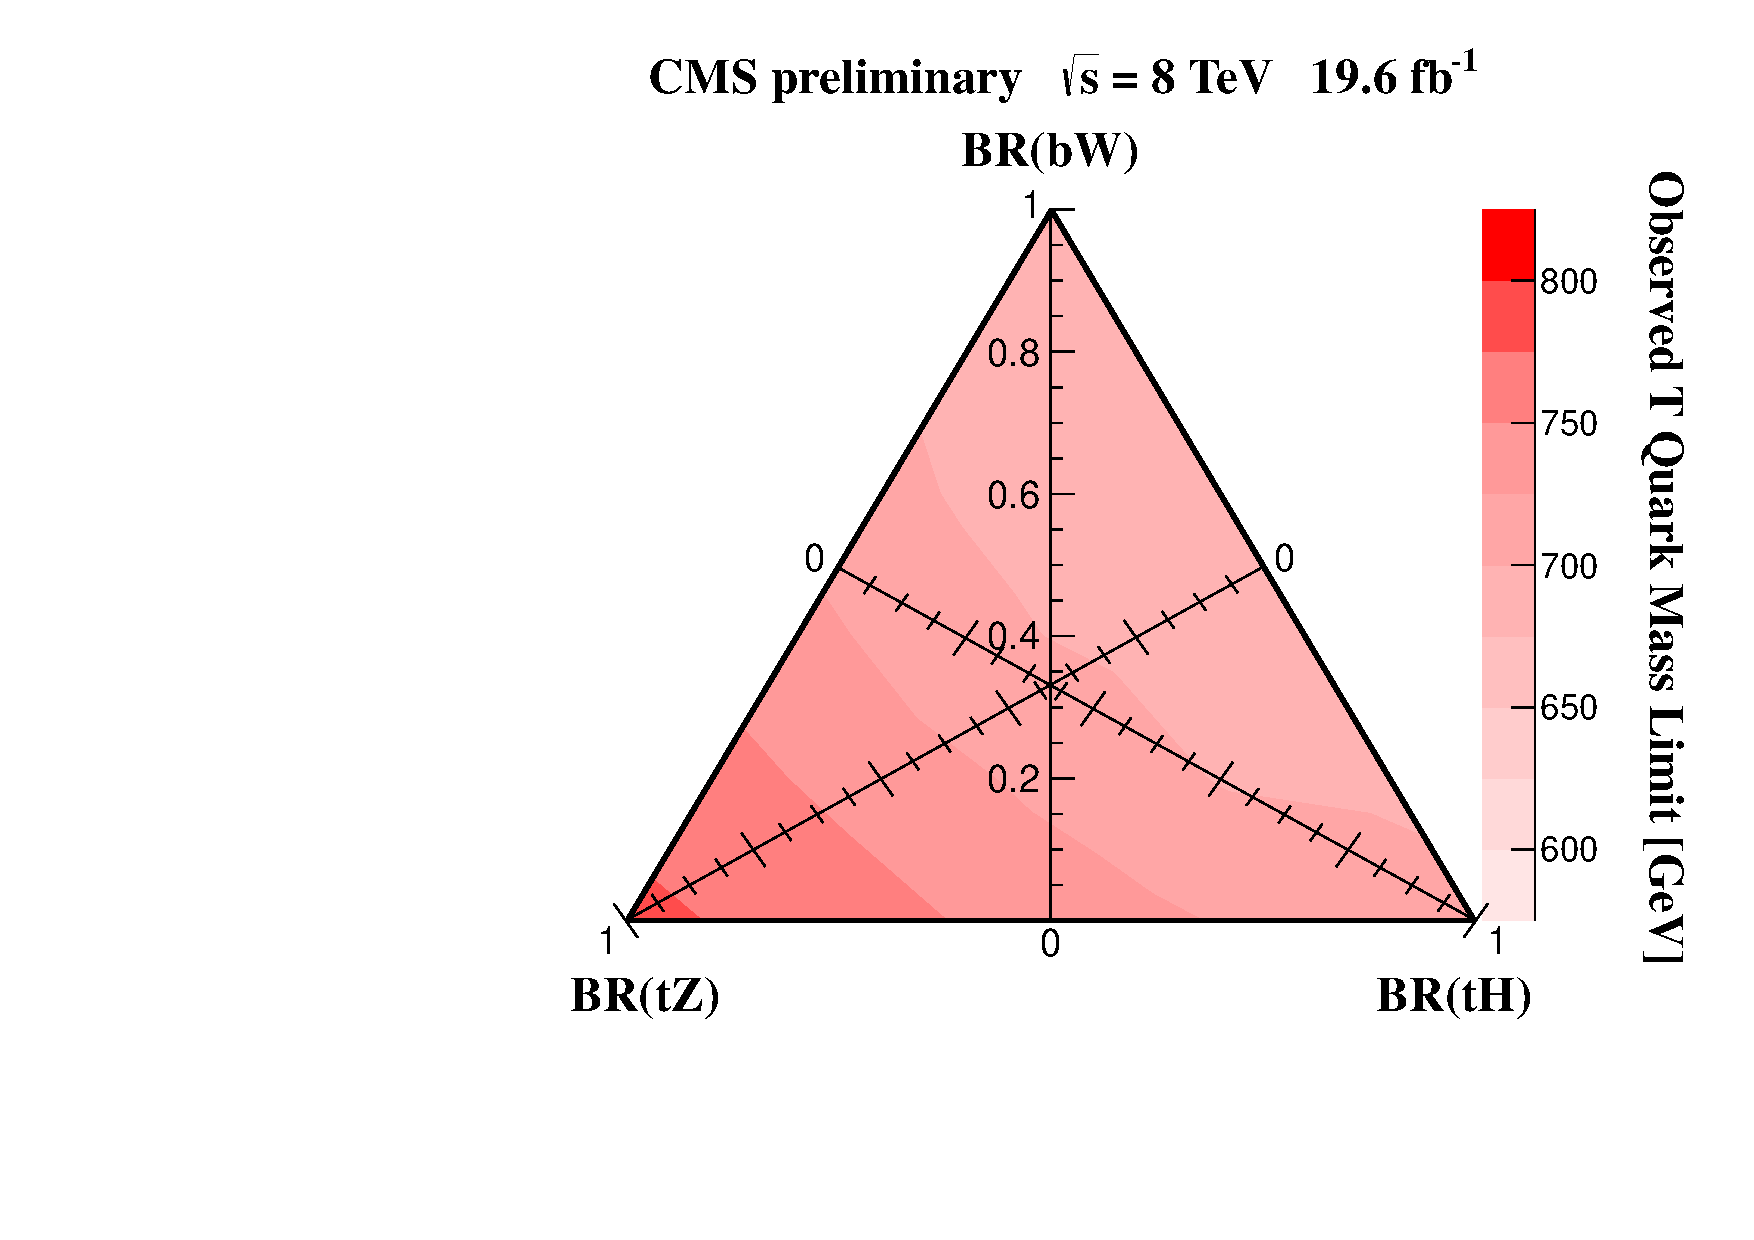
\includegraphics[width=.8\textwidth]{pics/cms/triangle}
\end{minipage}\begin{minipage}{.4\textwidth}\centering

\begin{pgfpicture}{0.0\textwidth}{0.0\textheight}{1.\textwidth}{.6\textwidth}
   \begin{pgftranslate}{\pgfpoint{-0.05\textwidth}{-0.15\textheight}}
\pgfdeclareimage[interpolate=true,width=1.\textwidth]{tabTT}{pics/cms/tableTT}
 \pgfsetlinewidth{1.pt}
 \usebeamercolor[bg]{head/foot boxes}
 \pgfputat{\pgfxy(0.0,0.0)}{\pgfbox[left,base]{\pgfuseimage{tabTT}}}
 \pgfrect[stroke]{\pgfxy(0.2,3.4)}{\pgfxy(5,0.25)}
 \pgfputat{\pgfxy(-1.2,3.4)}{\pgfbox[left,base]{\cccolor ``doublet''}}
 \pgfputat{\pgfxy(-1.2,3.1)}{\pgfbox[left,base]{\cccolor 790 obs}}
 \pgfrect[stroke]{\pgfxy(0.2,1.4)}{\pgfxy(5,0.25)}
 \pgfputat{\pgfxy(-1.2,1.4)}{\pgfbox[left,base]{\cccolor ``singlet''}}
 \pgfputat{\pgfxy(-1.2,1.1)}{\pgfbox[left,base]{\cccolor 670 obs}}
 \pgfrect[stroke]{\pgfxy(0.2,0.)}{\pgfxy(5,0.25)}
 \pgfputat{\pgfxy(-1.2,0.)}{\pgfbox[left,base]{\cccolor ``chiral''}}
 \pgfputat{\pgfxy(-1.2,-0.3)}{\pgfbox[left,base]{\cccolor 740 obs}}
 \pgfrect[stroke]{\pgfxy(4,-0.05)}{\pgfxy(1,5.)}
\end{pgftranslate}
\end{pgfpicture}

\end{minipage}


\end{frame}

